\documentclass[a4paper,10pt]{article}
\usepackage[utf8]{inputenc}
\usepackage[english,czech]{babel}
\usepackage{makeidx}
\usepackage{url}
\usepackage{tikz}
\usepackage{float}
\usepackage{pdfpages}
\usepackage{amsfonts}
\usepackage{mdwlist}
\usepackage{xcolor}
\usepackage{listings}
\usepackage[utf8]{inputenc}
\usepackage[T1]{fontenc}
\usepackage{listingsutf8}
\usepackage{cite}
\usepackage{mdframed}



\newcommand{\ttt}[1]{\texttt{#1}}

\begin{document}
\title{IoT Akvárium}
\author{Martin Beránek}
\maketitle

\tableofcontents
\listoffigures
\listoftables

\section{Úvod}

Semestrální úloha má za cíl vytvořit ovladatelné akvárium, které bude schopné postarat se o~rybičky. Mezi základní vlastnosti\label{vlastn}, které je nutné spravovat, je:

\begin{itemize}
	\item Krmení,
	\item Rozsvědcení světla a zhasínání,
	\item Regulace vyhřívání,
	\item Kontrola výšky hladiny.
\end{itemize}

Údaje o~akváriu je nutné uchovávat pro statistiky. Pro potřeby upozornění je nutné neustále kontrolovat stav hladiny. Na základě toho je stanovena jednoduchá architektura obsahující server, který sbírá informace a logický obvod akvária tvořený platformou \texttt{Arduino}.

\begin{figure}[H]
  \centering
    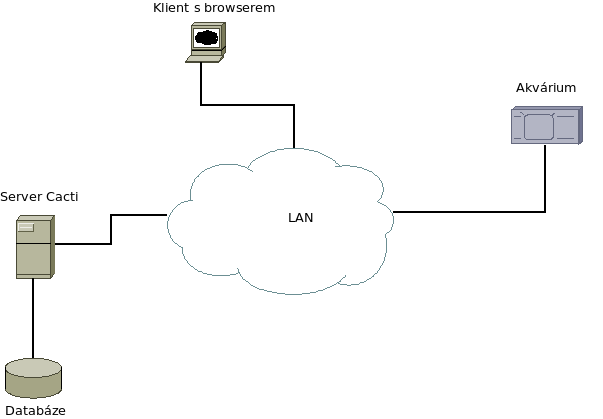
\includegraphics[width=1\textwidth]{net.png}
  \caption{Architektura}
  \label{char:arch}
\end{figure}

Pro vytváření grafů přímo na serveru slouží aplikace \texttt{Cacti}. Ta pomocí polleru spouští skript, který opakově otvírá \texttt{TCP} spojení na \texttt{Arduino} a zjisťuje současný stav. Na základě toho vytváří pomocí \texttt{RRDTool} graf.

\section{Popis součástek}

Na základě definovaných vlastností (\ref{vlastn}) byly vybrány následující součástky na platformu \ttt{Arduino}:

\begin{description}
	\item[Krokový motor] -- pro otáčení bubínku s~krmením pro rybičky.
	\item[Relé] -- pro spínání již vestavěného vytápění, osvětlení a filtru.
	\item[Teploměř] -- pro měření teploty vody v~akváriu.
	\item[RTC] -- (\uv{Real-time clock}) pro reálný čas.
	\item[Bójka jako spínač hladiny] -- v~případě, že v~akváriu klesá hladina vody, sepne se bójka a \ttt{Arduino} uloží hodnotu o~problému.
	\item[Ethernet shield] -- pro komunikaci se serverem pomocí \ttt{TCP} komunikace.
\end{description}

Vzhledem k~tomu, že otáčení bubínku s~krmením pro rybičky nevyžaduje nějakou větší sílu, je použit jednoduchý krokový motor \ttt{28BYJ-48}. Ten je připevněn na bubínek a je řízen driverem \ttt{ULN2003}. 

\begin{figure}[H]
  \centering
    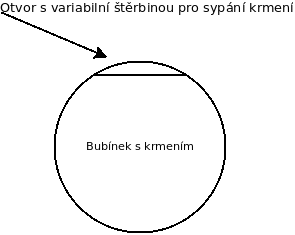
\includegraphics[width=0.7\textwidth]{krmeni.png}
  \caption{Diagram bubínku s~krmením}
  \label{char:bub}
\end{figure}

Pro spínání aktivních součástí akvária, které v~něm už jsou zabudované, slouží relé. Relé jsou připojena na napájení ze sítě. Spínané součásti jsou: osvětlení, vyhřívání a filtr.

Teploměr musí být vodotěsný. V~této práci je použita teplotní sonda s~čidlem \ttt{DS18B20}. Ta je ponořena v~akváriu na místě, kde je velký proud vody, aby rychle reagovala na změny teploty.

\ttt{Arduino} neobsahuje žádný modul reálného času. Kvůli nestabilnímu krystalu není ani možné měřit přesné časové intervaly. Na základě toho je připojen k~\ttt{Arduinu} obvod \ttt{RTC} s~obvodem \ttt{DS3231}.

\section{Schéma}

Na základě výběru součástek je vytvořeno schéma celé zapojení obvodu:

\begin{figure}[H]
  \centering
    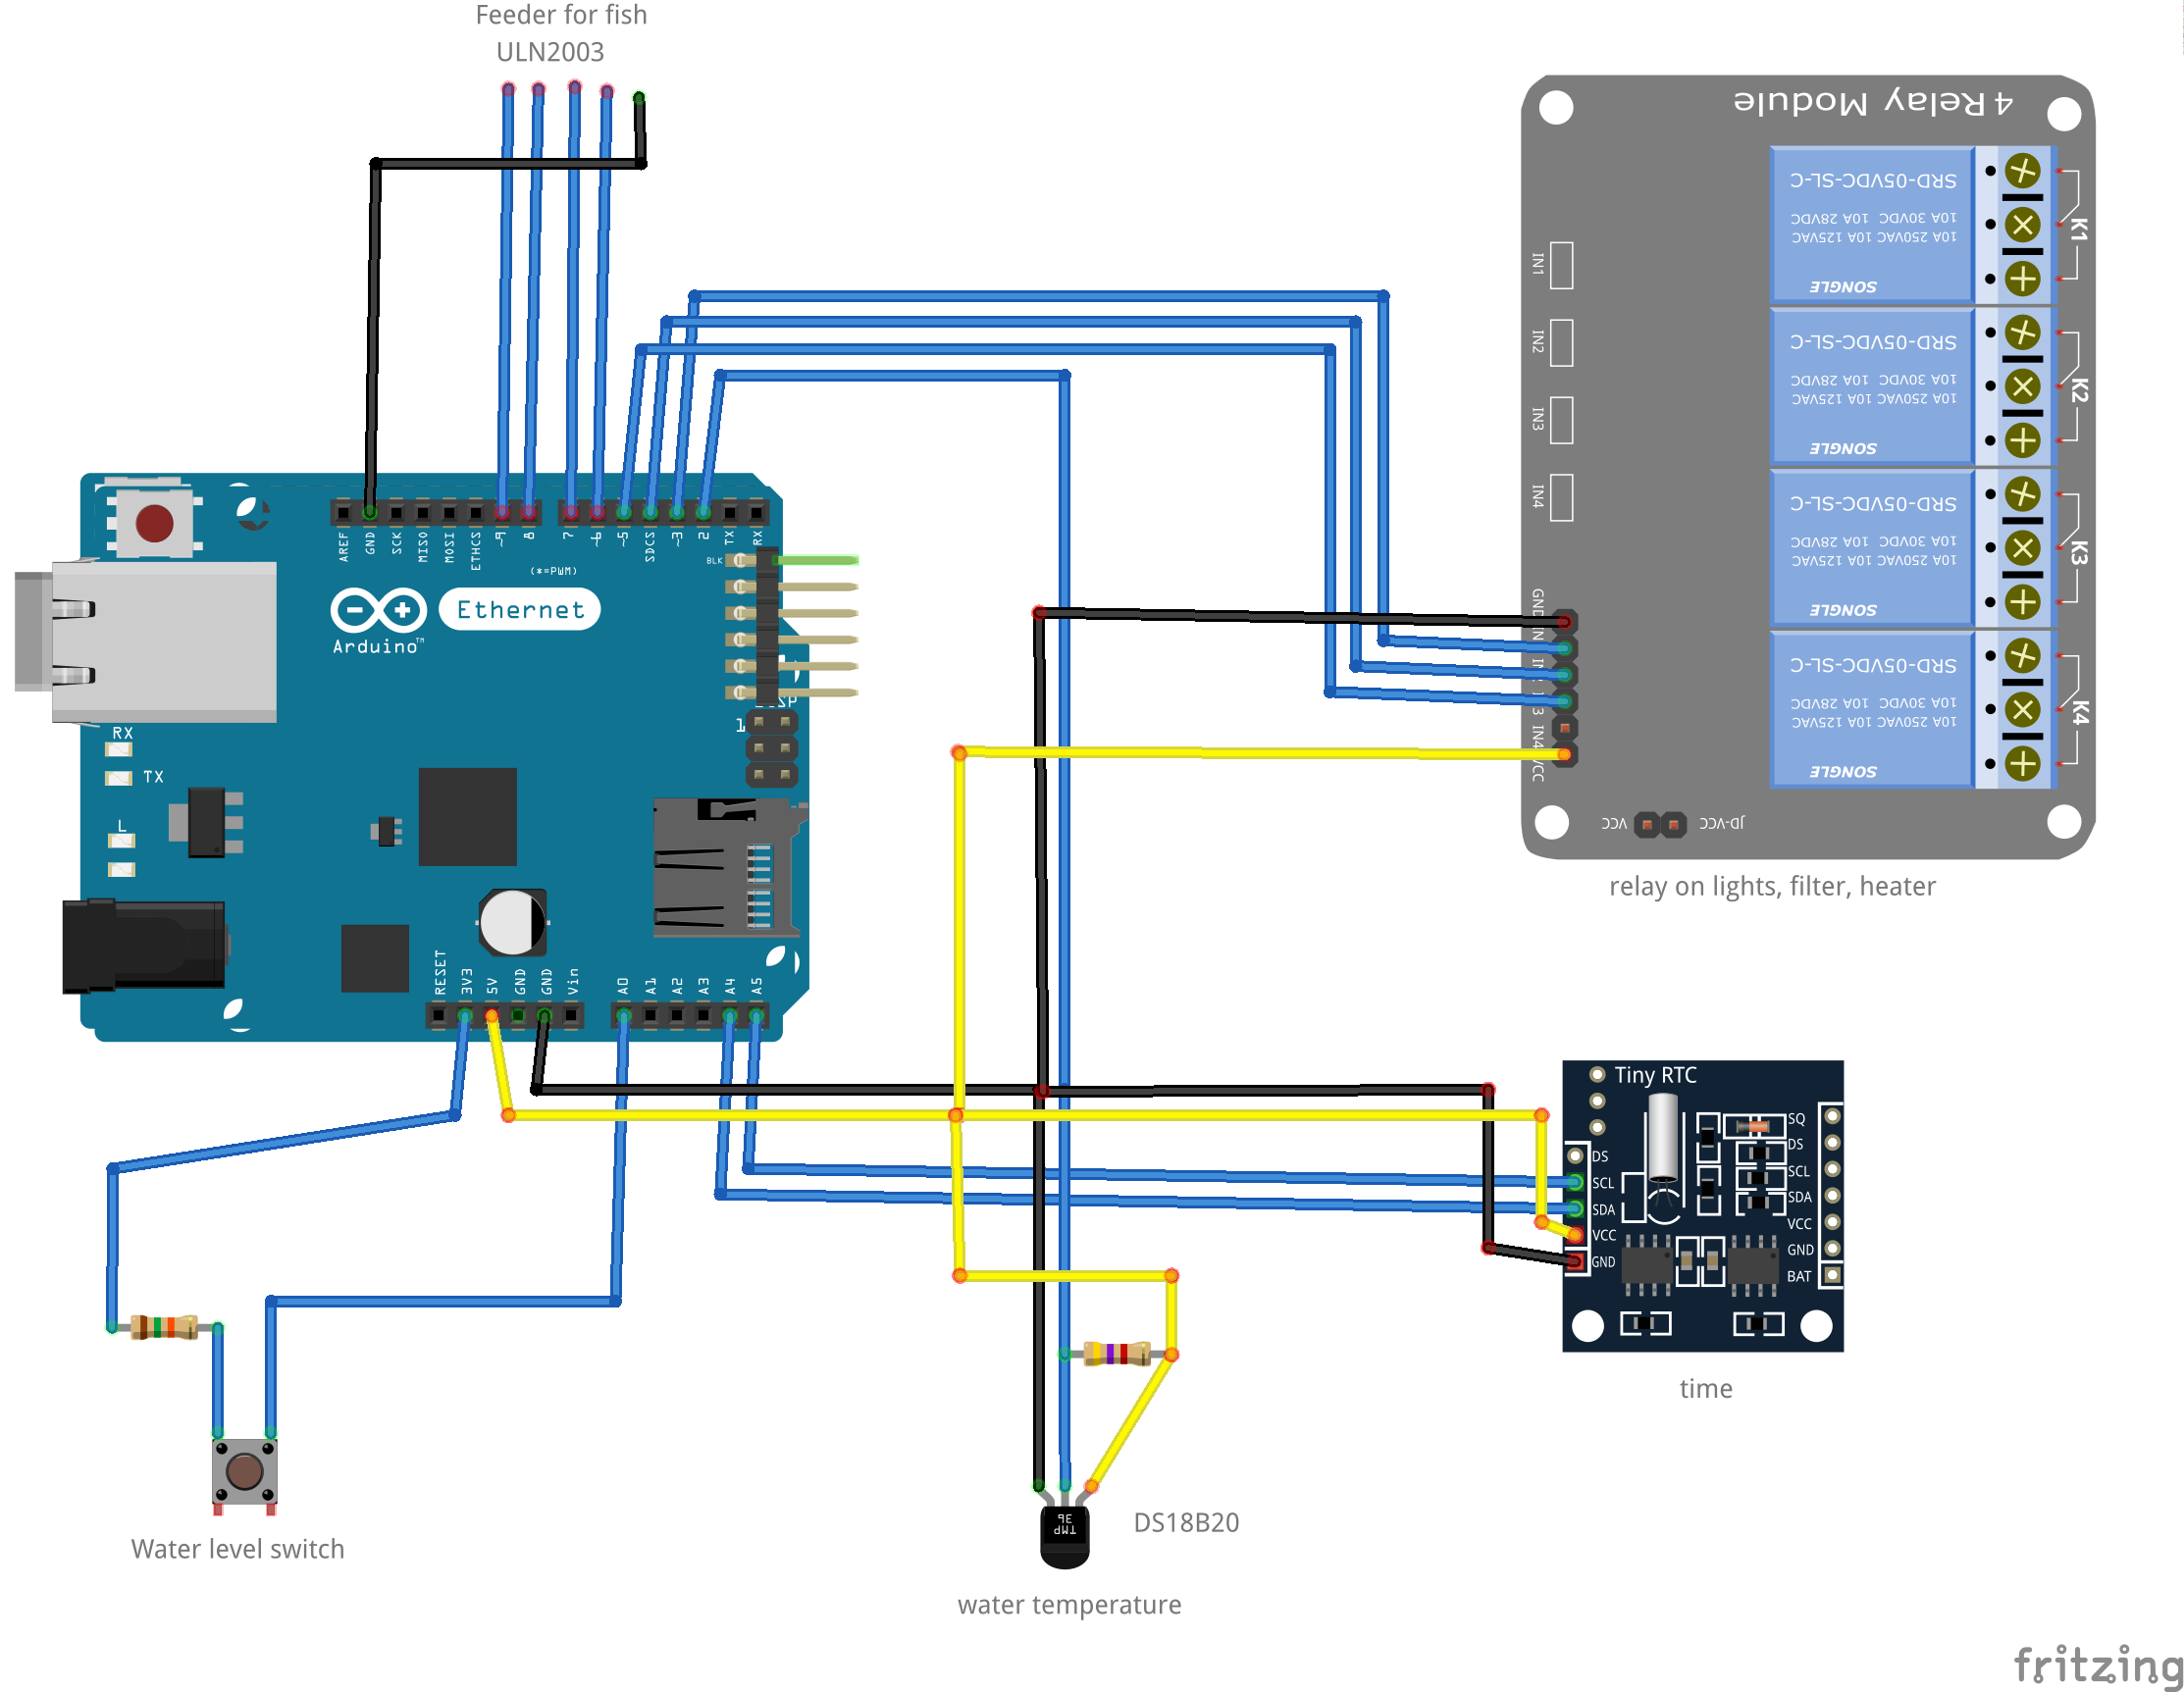
\includegraphics[width=1\textwidth]{schema_bb.png}
  \caption{Schéma zapojení součástek}
  \label{char:scbb}
\end{figure}

\section{Aplikace}

\section{Komunikace}

Komunikace probíhá pomocí \ttt{TCP/IP} komunikace. \ttt{Arduino} naslouchá na na pevně zadané \ttt{IP} adrese. Na základě příkazů dlouhých několik bytů aplikace na \ttt{Arduinu} vytvoří zprávu a odešle jí v~rámci komunikace. Příkazy, které \ttt{Arduino} zná jsou v~následujícím seznamu:

\begin{verbatim}
GZ - vrátí stav spínače hladiny
GM - vrátí teplotu, která má být v~akváriu
GT - vrátí reálnou teplotu v~akváriu
GL - vrátí stav relé obsluhující svétlo
GF - vrátí stav relé obsluhující filtr
GH - vrátí stav relé obsluhující vytápění
GN - vrátí reálný čas Arduina
GP - otočí bubínkem s~krmením
GW - vrátí čas, kdy má Arduino zapnout světla v~akváriu
GE - vrátí čas, kdy má Arduino vypnout světla v~akváriu
GK - vrátí čas, kdy má Arduino nakrmit rybičky

SE hh mm - nastaví čas, kdy má Arduino vypnout světla v~akváriu
SW hh mm - nastaví čas, kdy má Arduino zapnout světla v~akváriu
SF hh mm - nastaví čas, kdy má Arduino nakrmit rybičky
ST nn - nastaví teplotu v~akváriu, které ma Arduino udržovat
SN -- nastaví čas pomocí NTP serveru
\end{verbatim}

V~případě, že \ttt{Arduino} nemá nastavený správný čas, vrací příkaz \ttt{GN} samé nuly. Pomocí příkazu \ttt{SN} \ttt{Arduino} zavolá \ttt{NTP} server a nastaví si čas podle času na \ttt{NTP}. Výstup nastaveného času může vypadat takto:

\begin{verbatim}
Trying 10.0.0.173...
Connected to 10.0.0.173.
Escape character is '^]'.
SN
8:36:50 4/5/16 Day of week: Wednesday
Connection closed by foreign host.
\end{verbatim}

\section{Načasování}

Všechny časovače pracují se strukturou obsahující binární proměnnou, které hlídá, aby v~intervalu nedošlo k~vypnutí nebo zapnutí vícekrát. 

\begin{verbatim}
struct Tmr{
  byte h;
  byte m;
  byte done;
};
\end{verbatim}

Časovač pracuje pouze s~hodinou a minutou. V~případě přepnutí je nastavena i proměnná \ttt{done}. K~jejímu navrácení do původní podoby musí uběhnout časový interval zvolené minuty.

\begin{verbatim}
void feedFish(){
  if (minute == feedt.m && hour == feedt.h && feedt.done == true){
    turnAround();
    feedt.done = false;
  }else if (minute != feedt.m  && feedt.done == false){
    feedt.done = true;
  }
}
\end{verbatim}

\section{Čtení senzorů}

\subsection{Teplota}

Teploměr pro měření je \ttt{DS18S20}. Komunikace s \ttt{Arduino} probíhá pomocí protokolu \ttt{OneWire}. Načítání probíhá pomocí zavolání senzoru na adrese \cite{dscd}. Potom jsou načteny byty, které vystaví senzor. Ty jsou upraveny do podoby jednoho \ttt{float}.

\begin{verbatim}
float getTemp(){
 byte data[12]; // data
 byte addr[8]; // adresa 

 if ( !ds.search(addr)) {
   ds.reset_search(); // hledání senzoru
   return -1000;
 }

 if ( OneWire::crc8( addr, 7) != addr[7]) {
   Serial.println("CRC is not valid!"); // kontrola CRC
   return -1000;
 }

 if ( addr[0] != 0x10 && addr[0] != 0x28) {
   Serial.print("Device is not recognized");
   return -1000;
 }

 ds.reset();
 ds.select(addr);
 ds.write(0x44,1); // Začátek komunikace

 byte present = ds.reset();
 ds.select(addr);  
 ds.write(0xBE);

 for (int i = 0; i < 9; i++) { // Načítání dat
  data[i] = ds.read();
 }
 
 ds.reset_search();
 
 byte MSB = data[1];
 byte LSB = data[0];

 float tempRead = ((MSB << 8) | LSB); // převod načtené teploty
 float TemperatureSum = tempRead / 16;
 
 return TemperatureSum;
 
}
\end{verbatim}

\subsection{Spínací plovák}

Jelikož už na \ttt{Arduinu} nezbyl žádný digitální \ttt{GPIO}. Byl pro spínač použit analogový vstup. Měření musí proběhnout tedy několikrát, protože i při sepnutém plováku může \ttt{AD} převodník vrátit nulu. Server tedy při měření zasílá hned několik dotazů.

\ttt{Arduino} tedy jen čte stav analogového vstupu:

\begin{verbatim}
void initSurface(){
	pinMode(SWITCH_SUR, INPUT);
}

int getSurface(){
  int buttonState = analogRead(SWITCH_SUR);
  if (buttonState > 0)
    return true;
  else
    return false;
}
\end{verbatim}

\subsection{Relé}


\section{Komunikace s \ttt{CACTI}}

\ttt{CACTI} je služba, která je primárně určená ke sběru dat o zařízeních na síti. Na základě načtených dat potom vytváří pomocí \ttt{RRDTool} grafy. V tomto případě se vytváří graf teploty v akváriu. V případě, že vytápění a teploměr pracují v pořádku, graf by měl být konstantní. Odběr dat z \ttt{Arduino} probíhá pomocí skriptu v jazyce \ttt{Python}:

\begin{verbatim}
#!/usr/bin/python
from __future__ import print_function
import socket

HOST = '10.0.0.173'    # The remote host
PORT = 9011              # The same port as used by the server
s = socket.socket(socket.AF_INET, socket.SOCK_STREAM)
s.connect((HOST, PORT))
s.sendall('GT\r\n')
data = s.recv(10)
s.close()
print('Temperature:' + str(data),end='')
\end{verbatim}

Výsledný graf jasně ukazuje, že teplota kolísá mezi dvěma stupni. Kolísání způsobuje otevřené okno na noc, které vodu ochladí a vytápění vždy teplotu postupně dorovná. K datu psaní této práce vypadá graf takto:


\begin{figure}[H]
  \centering
    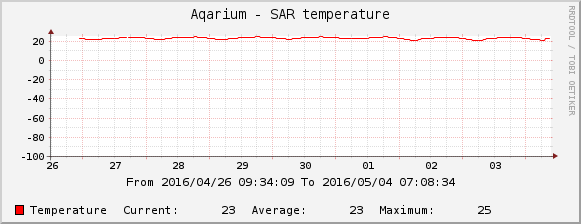
\includegraphics[width=1\textwidth]{graph.png}
  \caption{Graf teploty v akváriu}
  \label{char:temps}
\end{figure}


\section{Závěr}

\bibliographystyle{csn690}
\bibliography{literatura}


\end{document}
